\documentclass{article}

\usepackage{geometry}
\usepackage{multicol}
\usepackage{fixltx2e}
\usepackage{url}


\usepackage{Sweave}
\begin{document}
\Sconcordance{concordance:mapAndDensity.tex:mapAndDensity.Rnw:%
1 8 1 1 0 2 1 1 8 19 1 1 8 1 3 15 1 1 12 1 2 13 1 1 17 1 3 5 1 1 2 1 0 %
1 1 1 2 1 1 1 2 1 1 1 2 1 1 1 2 2 1 2 2 9 1 2 2 6 1 1 4 6 1 1 2 3 1 1 3 %
2 0 1 1 1 3 1 0 1 6 5 0 1 2 3 1 1 2 9 1 1 3 1 0 1 2 1 1 1 2 2 1 1 3 1 0 %
1 4 1 0 1 2 1 0 7 1 1 5 4 0 1 4 3 0 1 2 1 1 4 0 1 3}




\newgeometry{margin=2.5cm}

\begin{center}
\begin{huge}
Issues raised at Haiti project meeting (Apr 11, 2014) \\
\end{huge}

\begin{small}
Joe Brew
\end{small}

\end{center}
\setkeys{Gin}{width=0.5\textwidth}

\begin{multicols}{2}
\subsection*{Does Carrefour's southern boundary extend to the sea?}
No. Carrefour is border by Jacmel to the south and Kenscoff to the southeast.\\

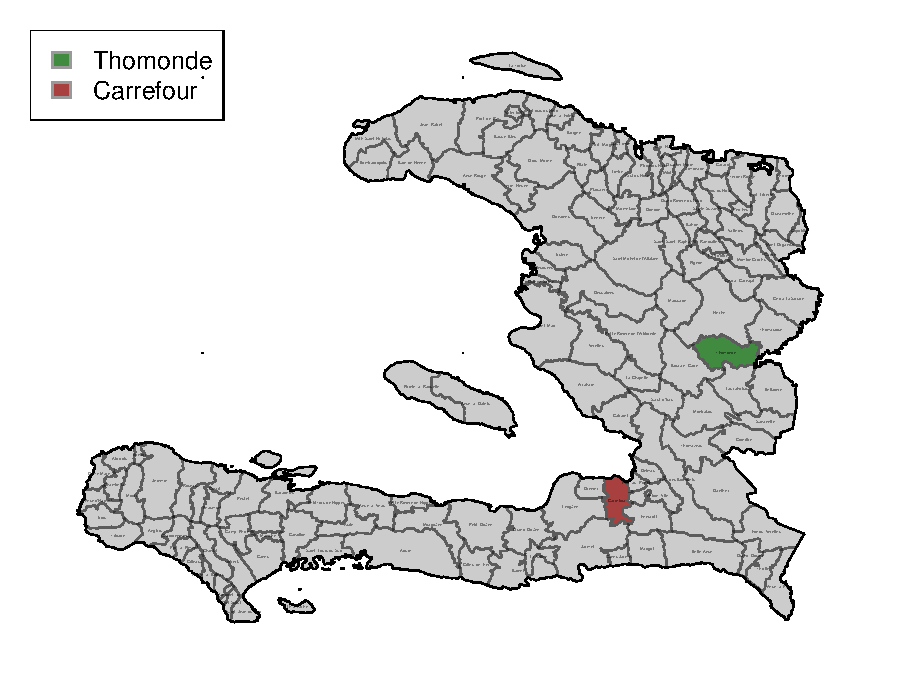
\includegraphics{mapAndDensity-002}
\footnote{Shapefile obtained from Global Administrative Boundaries Database, version 2: \url{http://www.gadm.org/country, and modified in R}}
%\vfill
%\columbreak


\subsection*{How many police districts are there in Carrefour?}
No clear answer.  Given that its part of the d�partement de l'ouest, Carrefour falls under the the DDO branch of the PNH (national police).  I called to ask about subdivisions within Carrefour and was told that the police districts operate under sous-commisariats at the neighborhood level (ie, independent of anu municipal boundaries, such as those of Carrefour).  


\subsection*{What is the unemployment rate?}
The unemployment rate is 27.4\%.  Among women, it is 32.1\% (23.4\% among men).  Unemployment is greatest among young people (61.9\% for 15-19 year-olds and 50\% among 20-24 year-olds).  Unemployment in the Port-au-Prince metropolitan area is 45.\%.  \footnote{"Force de travail", p. 322. \url{http://www.ihsi.ht/pdf/ecvh/ECVHVolumeI}}

\subsection*{What will we miss out on if we choose a small age range?}
If we exclude those  50 years of age or older, we miss out on 12.8\% of the total population, or 27.2\% of the adult population (defined here as older than 19).   If we exclude those 55 years of age or older, we miss out on 94.\% of the total population (20\% of the adult population).  If we exclude those 60 years of age or older, we miss out on 6.5\% of the total population (13.9\% of the adult population). If we exclude those 65 years of age or older, we miss out on 4.5\% of the total population (9.5\% of the adult population).   


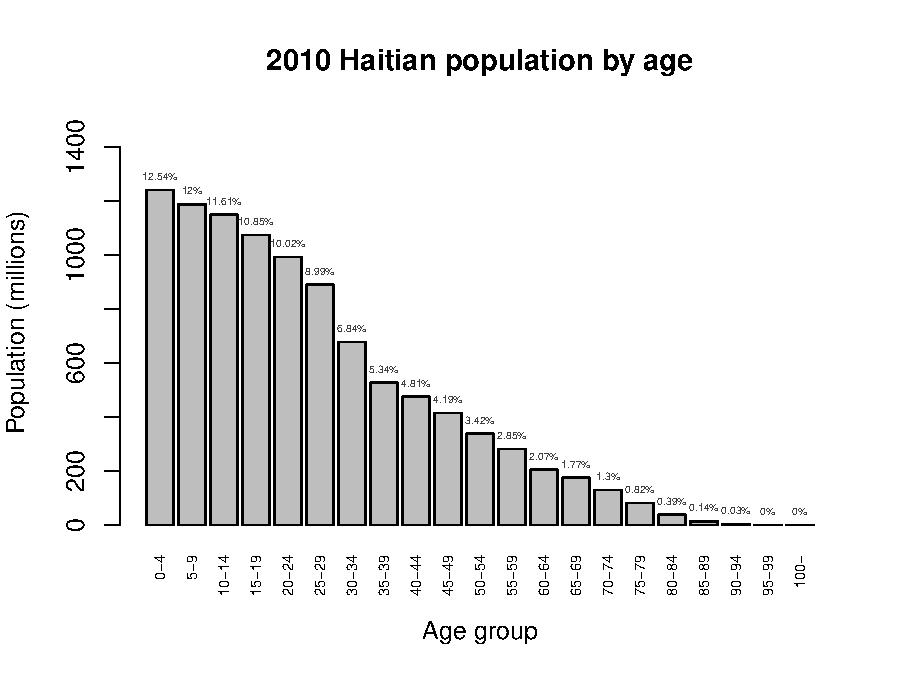
\includegraphics{mapAndDensity-003}
\footnote{\url{http://esa.un.org/unpd/wpp/unpp/panel_population.htm}}


\subsection*{What is our operational definition for "urban" and "rural"?}
The Institut Ha�tien de Statistique et d'Informatique uses the definitions for "rural" and "urban" devised by the 1997 Echantillon-Ma�tre d'Enqu�tes Multiples.\footnote{\url{http://www.ihsi.ht/pdf/EBCM/Methodologie_EBCM.pdf}}  Essentially, all 8 non-metropolitan d�partements are divided into two: their urban and rural parts.  I can find no further references to the what constitutes rural/urban in their approach. \\

However, I've mapped population density at the commune level (next page), which should at least give a pretty good idea of which areas can be considered urban/rural.  


\end{multicols}
\newpage

\begin{center}
\setkeys{Gin}{width=1.1\textwidth}
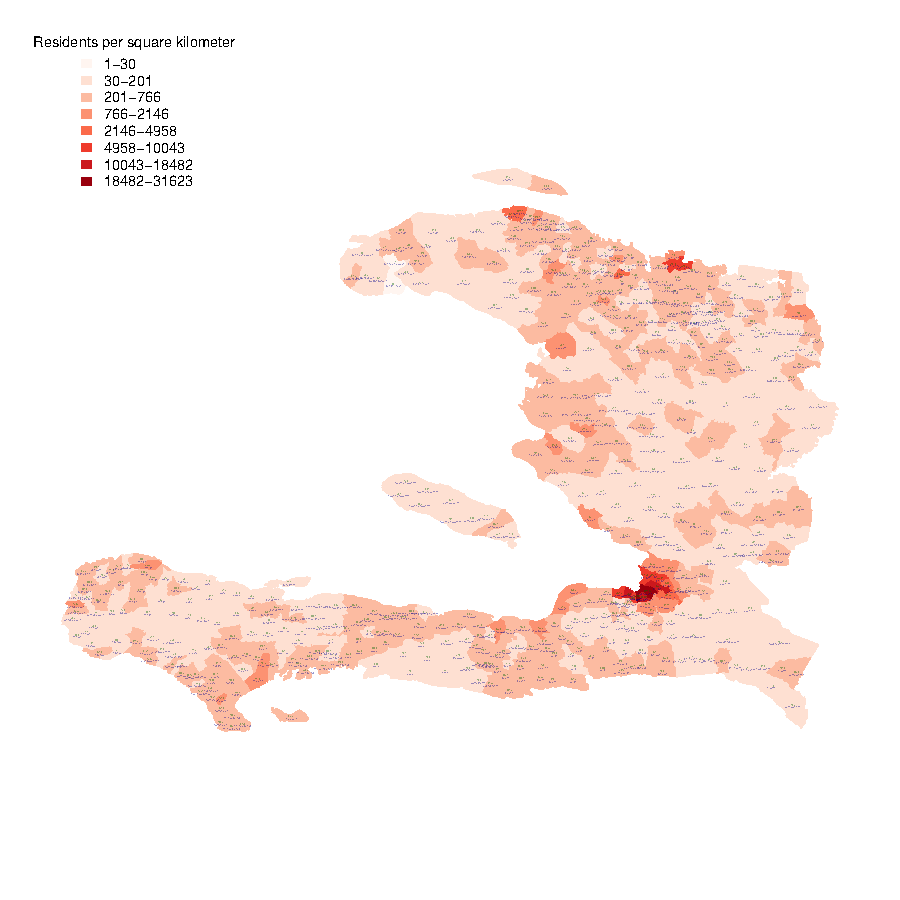
\includegraphics{mapAndDensity-004}
\footnote{Shapefile and population density obtained at: http://www.gvsu.edu/haitiwater/links-to-gis-data-for-haiti-9.htm}
\end{center}


\subsection*{R Code}

\begin{Schunk}
\begin{Sinput}
> load("E:/workingdirectory/gis/haiti/haiti0.RData")
> map0 <- gadm
> load("E:/workingdirectory/gis/haiti/haiti1.RData")
> map1 <- gadm
> load("E:/workingdirectory/gis/haiti/haiti2.RData")
> map2 <- gadm
> load("E:/workingdirectory/gis/haiti/haiti3.RData")
> map3 <- gadm
> map3$color <- adjustcolor("black", alpha.f=0.2)
> map3$color[which(grepl("Carrefour", map3$NAME_3)==TRUE)] <- adjustcolor("darkred", alpha.f=0.75)
> map3$color[which(grepl("Thomonde", map3$NAME_3)==TRUE)] <- adjustcolor("darkgreen", alpha.f=0.75)
> plot(map3, border=adjustcolor("black", alpha.f=0.5),  col=map3$color)
> labelpos <- data.frame(do.call(rbind, lapply(map3@polygons, function(x) x@labpt)))
> names(labelpos) <- c("x","y")                        
> map3@data <- data.frame(map3@data, labelpos)
> map3$labelpos <- labelpos
> map3$labelposx <- labelpos$x
> map3$labelposy <- labelpos$y
> zippy <- unique(sort(map3$NAME_3))
> zippy <- as.character(zippy)
> map3$text <- 1
> for (i in zippy){map3$text[which(map3$NAME_3 == i)] <- i }
> text(labelpos$x, labelpos$y, label=map3$text, cex=0.1, col=adjustcolor("black", alpha.f=0.4))
> library(maptools)
> library(maps)
> library(RColorBrewer)
> library(classInt)
> mapDen <- readShapePoly("E:/workingdirectory/gis/haiti/popDensity/Haiti_ADM3_stats.shp")
> plot(mapDen)
> summary(mapDen)
> plotvar<-(mapDen$POP_DENS)^(1/4.5)
> nclr<- 8 # number of bins (3-8)
> min<- floor(min(plotvar))
> max<- ceiling(max(plotvar))
> breaks<- (max-min) / nclr
> plotclr<- brewer.pal(nclr, "Reds")
> class<- classIntervals(plotvar, nclr, style ="fixed", fixedBreaks=seq(min, max, breaks))
> colcode<- findColours(class, plotclr)
> colcode2<-gsub(",","-", gsub("[[]|[)]|[]]","", names(attr(colcode, "table"))))
> colcode3 <- round(as.numeric(unlist(strsplit(colcode2, "-")))^4.5, digits=0)
> colcode4 <- c()
> for (i in seq(1, length(colcode3),2)){
+   colcode4[i] <- paste0(colcode3[i], "-", colcode3[i+1])
+ }
> colcode5 <- colcode4[seq(1, length(colcode4),2)]
> ### Plot the Map
> plot(mapDen, border=FALSE, fill=TRUE, col=colcode)# ONCE YOUVE DEFINED PLOT VAR
> ###Add a Legend
> legend("topleft",
+        legend = colcode5, 
+        title= "Residents per square kilometer",
+        fill=attr(colcode, "palette"),
+        cex= 0.56, bty="n", border=FALSE) 
> plot(map0, border=adjustcolor("black", alpha.f=0.3), add=TRUE)
> plot(map1, border=adjustcolor("black", alpha.f=0.3), add=TRUE)
> plot(map2, border=adjustcolor("black", alpha.f=0.3), add=TRUE)
> plot(map3, border=adjustcolor("black", alpha.f=0.3), add=TRUE)
> labelpos <- data.frame(do.call(rbind, lapply(mapDen@polygons, function(x) x@labpt)))
> names(labelpos) <- c("x","y")                        
> mapDen@data <- data.frame(mapDen@data, labelpos)
> mapDen$labelpos <- labelpos
> mapDen$labelposx <- labelpos$x
> mapDen$labelposy <- labelpos$y
> zippy <- unique(sort(mapDen$POP_DENS))
> zippy <- as.character(zippy)
> mapDen$text <- 1
> for (i in zippy){mapDen$text[which(mapDen$POP_DENS == i)] <- i }
> text(labelpos$x, labelpos$y, label=round(mapDen$text, digits=1), 
+      cex=0.1, col=adjustcolor("black", alpha.f=0.4))
> zippy2 <- unique(sort(mapDen$COMMUNE))
> zippy2 <- as.character(zippy2)
> mapDen$COMMUNE <- as.character(mapDen$COMMUNE)
> mapDen$text2 <- 1
> for (i in zippy2){mapDen$text2[which(mapDen$COMMUNE == i)] <- i }
> text(labelpos$x, labelpos$y, label=mapDen$text2, , 
+      cex=0.5, col=adjustcolor("black", alpha.f=0.4))
> ########UN POP
> unPop <- read.csv("E:/workingdirectory/haiti/meeting2014-04-11/unPopulation2012.csv", skip=16)
> unPop <- unPop[which(unPop$Major.area..region..country.or.area.. == "Haiti" &
+                        unPop$Reference.date..as.of.1.July. == 2010),]
> unPop <- unPop[colnames(unPop[which(grepl("X",colnames(unPop)))])]
> row.names(unPop) <-NULL
> unPop <- as.data.frame(t(unPop))
> colnames(unPop) <- "number"
> unPop$age <- row.names(unPop)
> row.names(unPop) <- NULL
> unPop <- unPop[which(unPop$age != "X80."),]
> mybp <- barplot(as.numeric(gsub(" ", "", unPop$number)), 
+                 names.arg=gsub("[.]", "-", gsub("X", "", unPop$age)),
+                 cex.names=0.6,
+                 las=3,
+                 xlab="Population (millions)", ylim=c(0, 1500))
> text(x=mybp[,1], y=as.numeric(gsub(" ", "", unPop$number))+50,
+      label = paste0(round(as.numeric(gsub(" ", "", unPop$number)) / 
+        sum(as.numeric(gsub(" ", "", unPop$number)))*100, digits=2), "%"),
+      cex=0.55, col=adjustcolor("black", alpha.f=0.75))
> unPop$age2 <- as.numeric(gsub(" ", "", unPop$number))
> save.image("E:/workingdirectory/haiti/meeting2014-04-11/mapAndDensity.RData")
> 
\end{Sinput}
\end{Schunk}
\end{document}
